% This file was created with tikzplotlib v0.10.1.
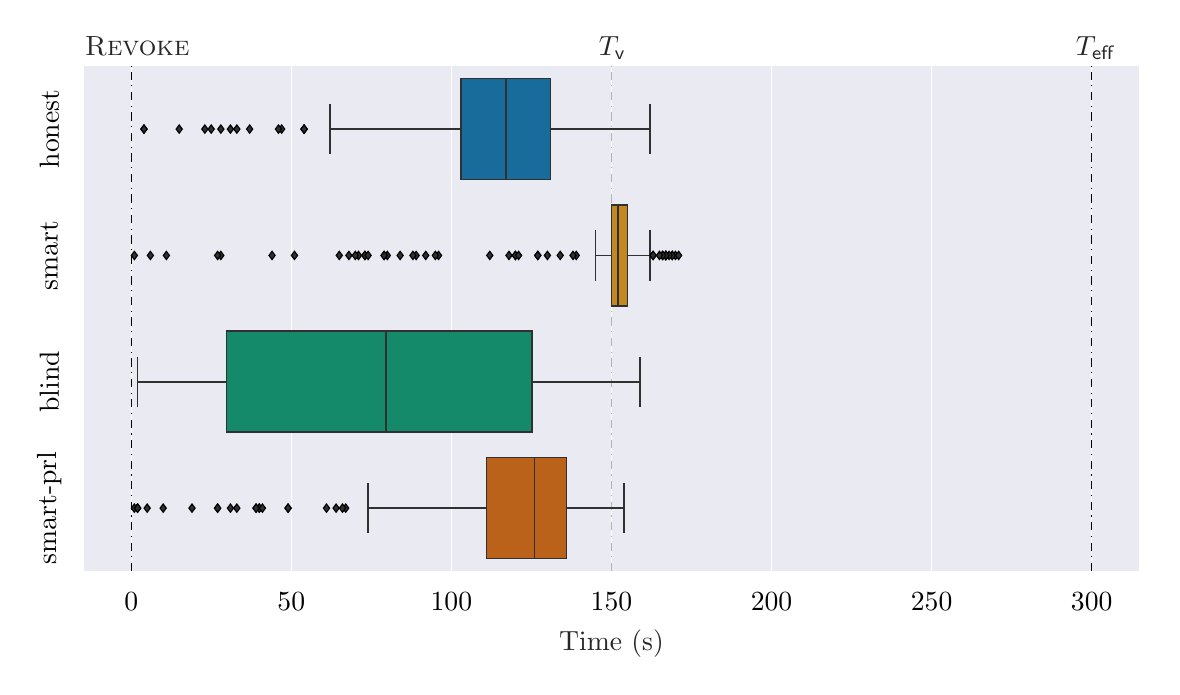
\begin{tikzpicture}

\definecolor{chocolate1869726}{RGB}{186,97,26}
\definecolor{darkgoldenrod19413532}{RGB}{194,135,32}
\definecolor{darkslategray38}{RGB}{38,38,38}
\definecolor{darkslategray48}{RGB}{48,48,48}
\definecolor{lavender234234242}{RGB}{234,234,242}
\definecolor{seagreen21138106}{RGB}{21,138,106}
\definecolor{teal23108155}{RGB}{23,108,155}

\begin{axis}[
clip=false,
axis background/.style={fill=lavender234234242},
axis line style={white},
height=8cm,
minor xtick={},
minor ytick={},
tick align=outside,
width=15cm,
x grid style={white},
xlabel=\textcolor{darkslategray38}{Time (s)},
xmajorgrids,
xmajorticks=true,
xmin=-15, xmax=315,
xtick style={color=darkslategray38,draw=none},
xtick={-50,0,50,100,150,200,250,300,350},
y dir=reverse,
y grid style={white},
ymajorticks=true,
ymin=-0.5, ymax=3.5,
ytick style={color=darkslategray38,draw=none},
ytick={0,1,2,3},
yticklabel style={rotate=90.0,anchor=center,yshift=8pt},
yticklabels={honest,smart,blind,smart-prl}
]
% START VERTICAL LINES %
\addplot [dashdotted, black]
table {%
0 3.5
0 -0.5
};
\addplot [dashdotted, gray!60]
table {%
150 3.5
150 -0.5
};
\addplot [dashdotted, black]
table {%
300 3.5
300 -0.5
};
% END VERTICAL LINES %
\path [draw=darkslategray48, fill=teal23108155, semithick]
(axis cs:103,-0.4)
--(axis cs:103,0.4)
--(axis cs:131,0.4)
--(axis cs:131,-0.4)
--(axis cs:103,-0.4)
--cycle;
\path [draw=darkslategray48, fill=darkgoldenrod19413532, semithick]
(axis cs:150,0.6)
--(axis cs:150,1.4)
--(axis cs:155,1.4)
--(axis cs:155,0.6)
--(axis cs:150,0.6)
--cycle;
\path [draw=darkslategray48, fill=seagreen21138106, semithick]
(axis cs:29.75,1.6)
--(axis cs:29.75,2.4)
--(axis cs:125.25,2.4)
--(axis cs:125.25,1.6)
--(axis cs:29.75,1.6)
--cycle;
\path [draw=darkslategray48, fill=chocolate1869726, semithick]
(axis cs:111,2.6)
--(axis cs:111,3.4)
--(axis cs:136,3.4)
--(axis cs:136,2.6)
--(axis cs:111,2.6)
--cycle;
\addplot [semithick, darkslategray48]
table {%
103 0
62 0
};
\addplot [semithick, darkslategray48]
table {%
131 0
162 0
};
\addplot [semithick, darkslategray48]
table {%
62 -0.2
62 0.2
};
\addplot [semithick, darkslategray48]
table {%
162 -0.2
162 0.2
};
\addplot [black, mark=diamond*, mark size=1.5, mark options={solid,fill=darkslategray48}, only marks]
table {%
4 0
15 0
31 0
33 0
4 0
37 0
25 0
47 0
28 0
54 0
23 0
54 0
46 0
54 0
};
\addplot [semithick, darkslategray48]
table {%
150 1
145 1
};
\addplot [semithick, darkslategray48]
table {%
155 1
162 1
};
\addplot [semithick, darkslategray48]
table {%
145 0.8
145 1.2
};
\addplot [semithick, darkslategray48]
table {%
162 0.8
162 1.2
};
\addplot [black, mark=diamond*, mark size=1.5, mark options={solid,fill=darkslategray48}, only marks]
table {%
127 1
73 1
89 1
96 1
84 1
118 1
80 1
134 1
28 1
79 1
120 1
127 1
120 1
51 1
130 1
65 1
88 1
71 1
112 1
68 1
27 1
73 1
79 1
44 1
74 1
1 1
121 1
6 1
95 1
92 1
139 1
70 1
138 1
11 1
167 1
166 1
169 1
163 1
170 1
167 1
167 1
169 1
168 1
167 1
167 1
166 1
163 1
171 1
165 1
};
\addplot [semithick, darkslategray48]
table {%
29.75 2
2 2
};
\addplot [semithick, darkslategray48]
table {%
125.25 2
159 2
};
\addplot [semithick, darkslategray48]
table {%
2 1.8
2 2.2
};
\addplot [semithick, darkslategray48]
table {%
159 1.8
159 2.2
};
\addplot [semithick, darkslategray48]
table {%
111 3
74 3
};
\addplot [semithick, darkslategray48]
table {%
136 3
154 3
};
\addplot [semithick, darkslategray48]
table {%
74 2.8
74 3.2
};
\addplot [semithick, darkslategray48]
table {%
154 2.8
154 3.2
};
\addplot [black, mark=diamond*, mark size=1.5, mark options={solid,fill=darkslategray48}, only marks]
table {%
1 3
61 3
27 3
40 3
27 3
2 3
64 3
49 3
67 3
19 3
2 3
2 3
10 3
31 3
39 3
66 3
33 3
40 3
41 3
39 3
49 3
5 3
};
\addplot [semithick, darkslategray48]
table {%
117 -0.4
117 0.4
};
\addplot [semithick, darkslategray48]
table {%
152 0.6
152 1.4
};
\addplot [semithick, darkslategray48]
table {%
79.5 1.6
79.5 2.4
};
\addplot [semithick, darkslategray48]
table {%
126 2.6
126 3.4
};
\draw (axis cs:-17.5,-0.58) node[
  scale=1,
  anchor=base west,
  text=darkslategray38,
  rotate=0.0
]{\textsc{Revoke}};
\draw[dashed] (axis cs:143,-0.58) node[
  scale=1,
  anchor=base west,
  text=darkslategray38,
  rotate=0.0
]{$T_{\mathsf{v}}$};
\draw (axis cs:292,-0.58) node[
  scale=1,
  anchor=base west,
  text=darkslategray38,
  rotate=0.0
]{$T_{\mathsf{eff}}$};
\end{axis}

\end{tikzpicture}
